\documentclass{rapportENS}
\usepackage{lastpage}
\rfoot{\thepage  / \pageref{lastpage}}
\title{Title page}
\begin{document}

%----------- Informations du rapport ---------
\titre{Ensemble Domotique EnOcean}
\Departement{Département Mécatronique}
\annee{$1^{ère}$ année}
\sujet{Analyse de système mécatronique }
\enseignant{S. Gardette, O. Bordron,\\ Q. Delamare, Alyssia Dong,\\
R. Le Goff latimier}
\eleves{Adrien \textsc{Vigné} \\ Martin \textsc{Filliung}}

%----------- Initialisation -------------------
\fairemarges{Vigné-Filliung} %Afficher les marges
\fairepagedegarde %Créer la page de garde
%\rfoot{\thepage  / \pageref{lastPage}}
\tabledematieres %Créer la table de matières

%------------ Corps du rapport ----------------

\part{Système étudié}
 \section{Présentation du système}
 La domotique à pour but d'interconnecter des sous-systèmes à la base indépendant afin d'améliorer l'interaction de l'ensemble avec son utilisateur. Ces technologies se retrouvent principalement dans l'habitat grâce à des capteurs connectés, des passerelle de contrôle ainsi que des actionneur ou des boîtiers de commande afin d'automatiser certaines actions ou de créer des alertes ou routine pour assister l'utilisateur. Ces installations demande d'être penser a la conception de la maison ou d'entreprendre des modifications afin de pouvoir les adapter à une installation existante car ils nécessitent entre autre une source d'énergie et ont un encombrement non négligeable. L'objet de cette étude à vocation à paliers à ces défauts en proposant une solution sans fils,sans alimentation externe et relativement peu encombrant afin de s'ajouter simplement à toute installation existante sans grande contraintes. 
 
 \section{Caractéristique du système}
 \subsection{Objectifs du système:}

 Cette ensemble domotique est l'ensemble proposé par la société \textit{EnOcean} (figure \ref{fig:kit_enOcean})avec des modules utilisant le principe de récupération d'énergie afin de minimiser leur impacts sur l'installation déjà présente. Le principe de récupération d'énergie est de permettre une indépendance énergétiques des modules au travers de transducteurs, tout en remplissant leurs objectifs d'interconnexion. Deux technologies employées pour répondre à ce critère seront étudié dans ce rapport. 
 
 \begin{figure}[h!]
     \centering
     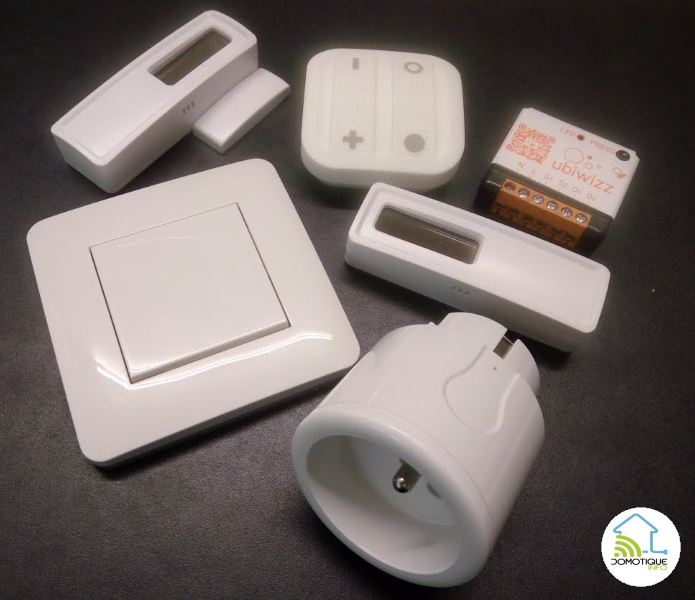
\includegraphics[scale=0.5]{kit_enocean.jpg}
     \caption{Ensemble de modules \textit{EnOcean}}
     \label{fig:kit_enOcean}
 \end{figure}
 
 \subsection{Cahier des charges}
 Les fonctions principales du kit sont représentées dans un diagrammes des interacteurs (Figure \ref{fig:Inter-acteurs}-\ref{tableau_cdcf}) dans le but ici de visualiser les principales fonctionnalité de l'objet d'études et les contraintes s'appliquant sur celui-ci.
 \begin{figure}[h!]
     \centering
     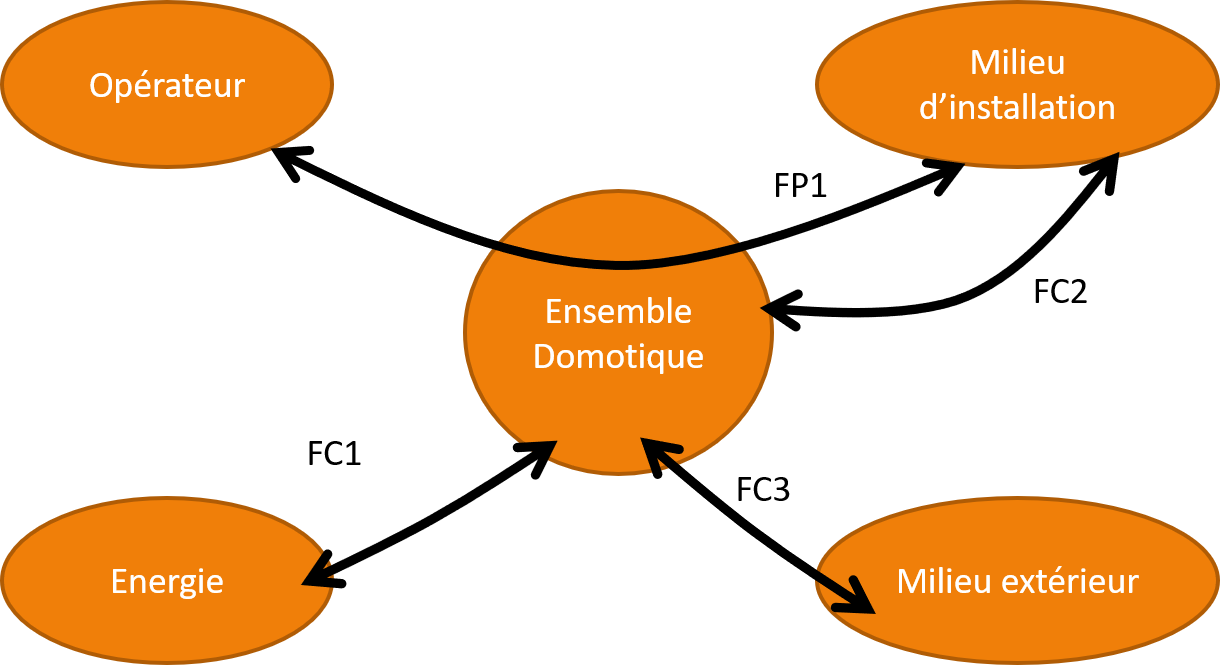
\includegraphics[width=0.9\linewidth]{Graphe_cdcdf.png}
     \caption{Diagramme des interacteurs}
     \label{fig:Inter-acteurs}
     \end{figure}
     
     \begin{figure}[h!]
         \centering
            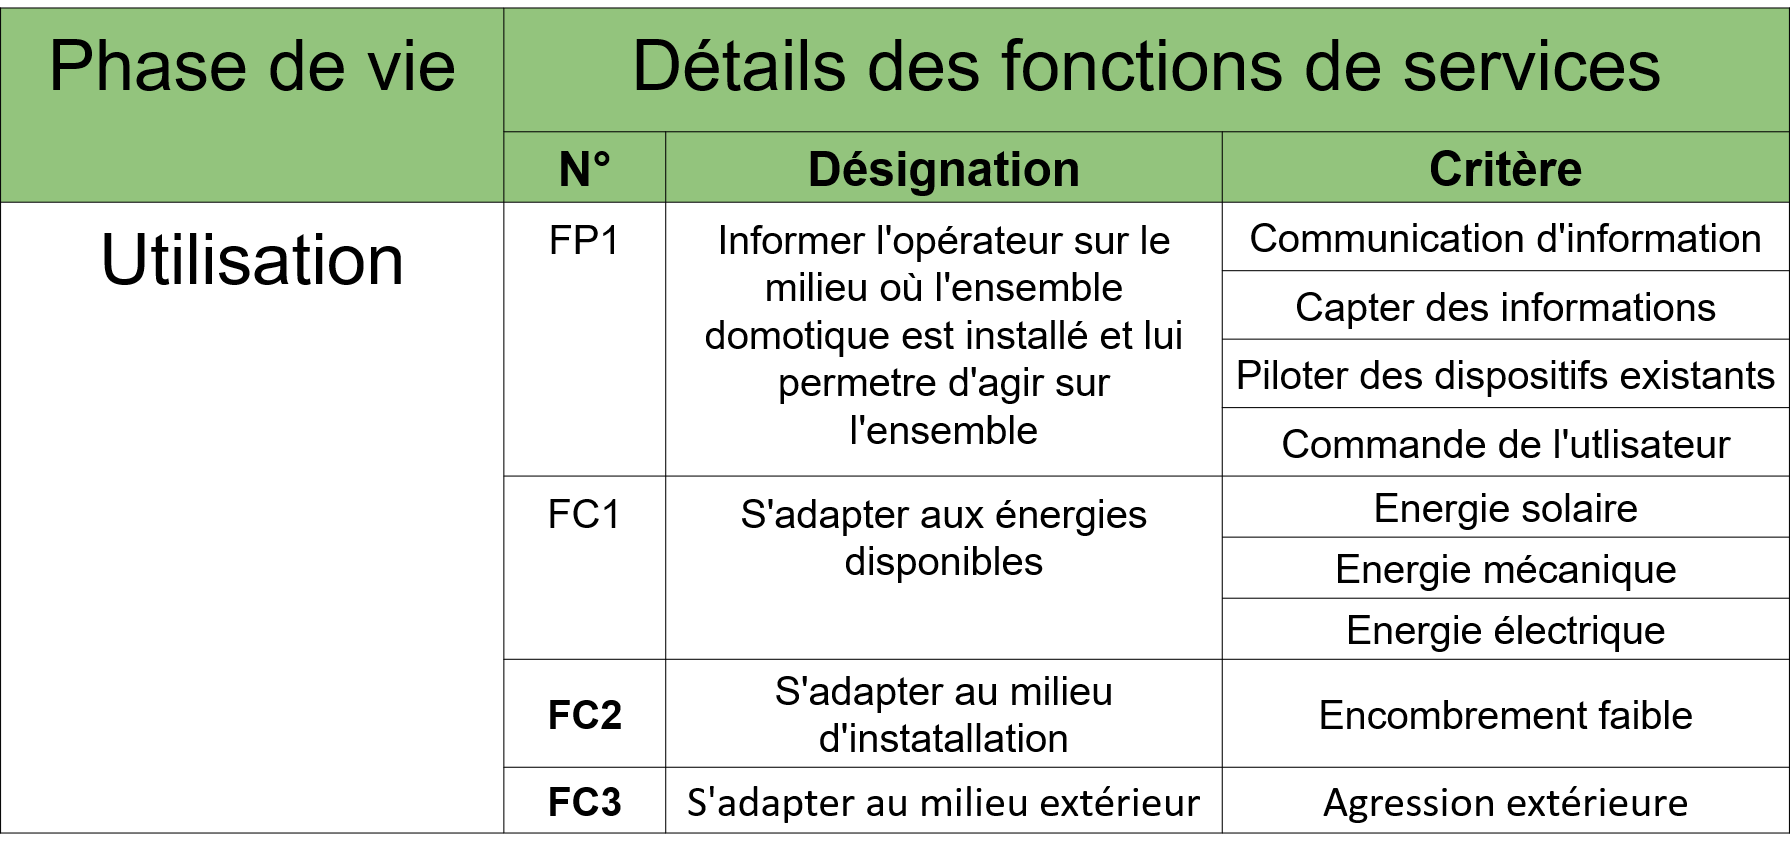
\includegraphics[width=\linewidth]{tableau_cdcf.png}
     \caption{Tableau du cahier des charges}
     \label{tableau_cdcf}
 \end{figure}
\subsubsection{Contraintes de conception}
La principales contrainte de conception de se système est la récupération d'énergie ceci imposant la conception ou l'utilisation d'un transducteur afin de récupéré l'énergie nécessaire au fonctionnement du dispositif. Une autre contraintes importante est l'adaptation du dispositif au milieu de l'installation notamment au niveau de son encombrement et sa faciliter de mise en place.   La résistance du matériel en milieu extérieurs implique aussi un minimum d'étanchéité de celui afin de supporter la pluie et l'humidité notamment.

\subsection{Ensemble disponibles pour l'étude}
Afin de mener cette analyse, le kit était composé de :
\begin{itemize}
\item commandes : 
\begin{itemize}
    \item interrupteurs sans fils pour gradateur
    \item interrupteurs sans fils monostable
\end{itemize}
\item Capteurs:
\begin{itemize}
    \item 2 capteurs de température
    \item 1 capteur d'ouverture de porte
\end{itemize}
\item actionneurs :
\begin{itemize}
    \item 1 prise piloté
    \item 1 contacteur piloté
\end{itemize}
\item passerelle : 
\begin{itemize}
    \item 1 passerelle wifi pour tableau électrique
    \item 1 paserelle pour \textit{Raspberry Pi}
    \item 2 passerelle USB
\end{itemize}
\item 1 kit de développement  
%  \item plusieurs interrupteurs sans piles 2 canaux;
%  \item 2 capteurs de température et d'hydrométrie;
%  \item 1 capteur d'ouverture de porte / fenêtre;
%  \item 1 contacteur piloté;
%  \item 1 passerelle \textit{EnOcean};
%  \item 1 kit de développement;
%  \item 1 passerelle pour \textit{Raspberry Pi}. 
\end{itemize}  
L'analyse à pour but de vérifier les fonctions principales et de contraintes identifier ainsi que les caractéristique techniques annoncées par le constructeur. 
 
%  \section{Caractéristiques du système}
 
%  Les modules proposés par \textit{ubiwizz} sur très variés (Environ 180 articles listés). Mis a notre disposition sont :
%  \begin{itemize}
%  \item plusieurs interrupteurs sans piles 2 canaux;
%  \item plusieurs capteurs de température et d'hydrométrie;
%  \item un capteur d'ouverture de porte / fenêtre;
%  \item un contacteur piloté;
%  \item une passerelle \textit{EnOcean};
%  \item un kit de développement;
%  \item une passerelle programmable \textit{Raspberry Pi}. 
% \end{itemize}  
 
%  \section{Contraintes de conception}
 
%  Les différents modules on pour contrainte d'être entièrement autonome une fois installés : ils ne doivent pas avoir à être rechargés, réinitialisés manuellement ou autrement manipulés pour bien fonctionner. De plus les modules doivent s'intégrer le plus facilement possible à l'environnement dans lequel on les place et donc être miniaturisés.
 
 \part{Étude}
 \paragraph{Objectifs:}  A partir des éléments disponibles l'analyse c'est concentré sur la caractérisation et la compréhension des systèmes de récupération d'énergie ainsi que la communication entre les modules et enfin la vérification des critères de portées des communications.
 
 \section{Récupération d'énergie}
 Une partie importante de l'analyse de ce système est l'analyse des technologies de récupération d'énergie. Dans les modules à disposition deux technologies sont utilisés, l'un utilise un transducteurs mécanique-électrique et l'autre optique-électronique. Le premier dispositif étudié est le convertisseur mécanique-électrique présent dans les interrupteurs de commande.
 \subsection{Transducteurs Mécanique-électrique}
 
 L'alimentation des interrupteurs sans fils est un circuit magnétique (aimant, fer et bobine, figure \ref{photocircuitmag}) dont la polarité de l'aimant peut être inversée grâce à une languette actionnée par l'utilisateur lorsqu'il presse le bouton (Figure \ref{schemacircuitmag}) il y a donc une partie mobile (en bleu et vert sur la figure \ref{schemacircuitmag} et une partie fixe dont l'aimant fait parti.
 
 \begin{figure}[h!]
 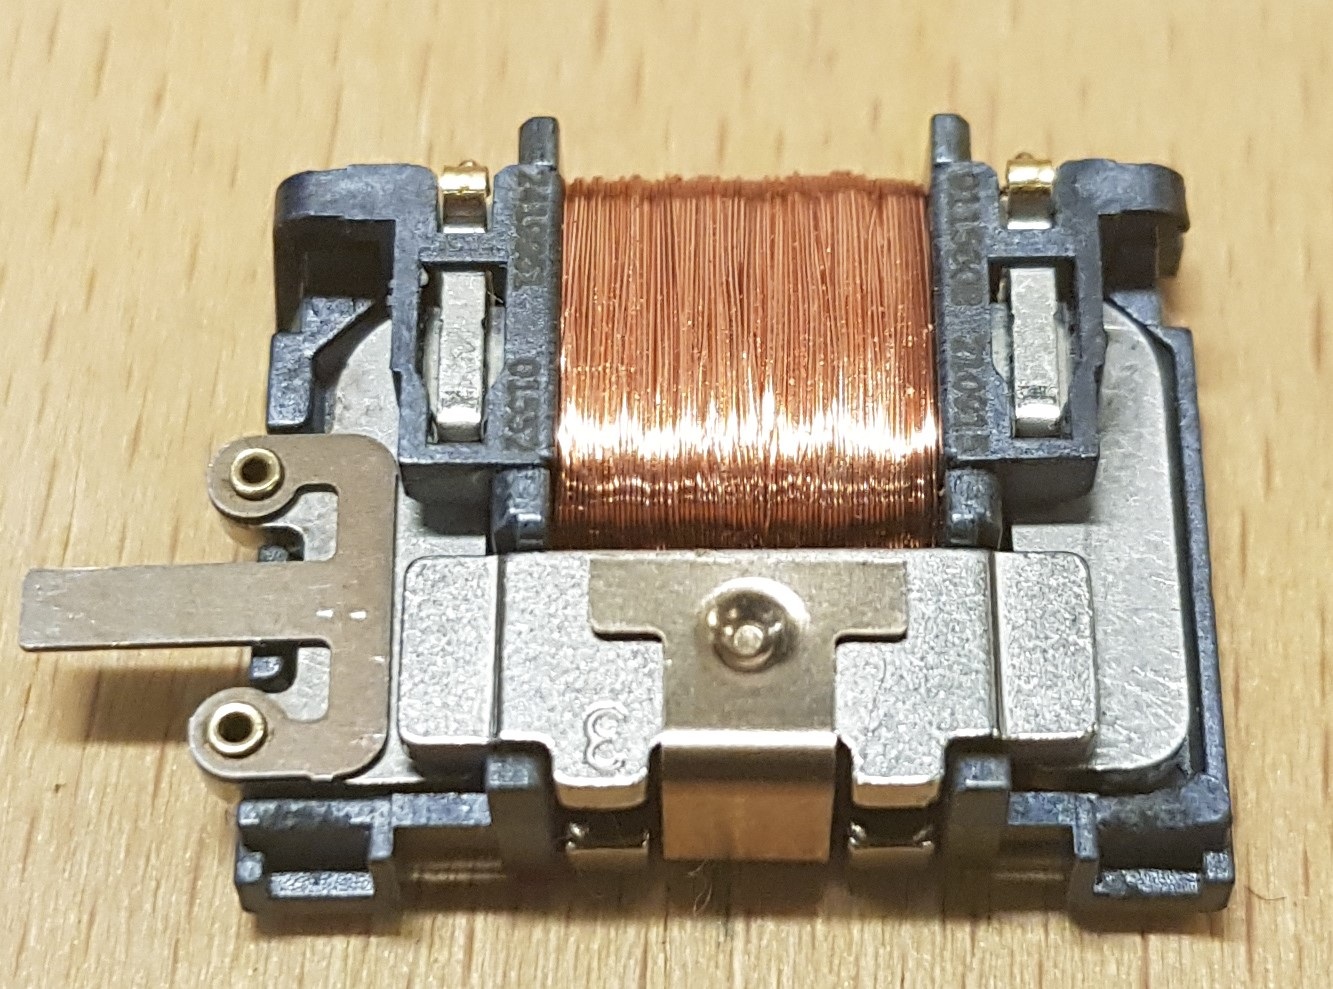
\includegraphics[width = .3\linewidth]{circuitmag.jpg}
 \centering
 \caption{Circuit magnétique alimentant les interrupteurs sans piles}
 \label{photocircuitmag}
 \end{figure}
 
 \begin{figure}[h!]
 \begin{subfigure}{.5\linewidth}
 \centering
 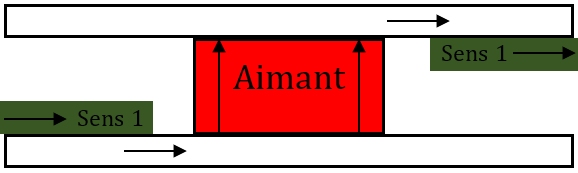
\includegraphics[width=.9\linewidth]{sens1.PNG}
 \caption{Sens 1 - direct}
 \label{sens1}
 \end{subfigure}
 \begin{subfigure}{.5\linewidth}
 \centering
 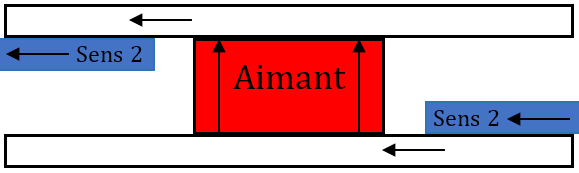
\includegraphics[width=.9\linewidth]{sens2.PNG}
 \caption{Sens 2 - inversé}
 \label{sens2}
 \end{subfigure}
 \caption{Différent positions du circuits magnétique}
 \label{schemacircuitmag}
 \end{figure}
 
 \subsubsection{Mesures et expériences}
 
 \subsubsection*{Mesure du pic de tension}
 
 
 
 \subsubsection*{Mesure du nombre de spires}
 
 Le nombre de spires est mesuré en faisant une seconde bobine sur le circuit magnétique dont on connais le nombre de spires $N_2 = 5$, le rapport des tensions $U_1$ et $U_2$ (figure \ref{nombredespire}) observés aux bornes des bobines sert a retrouver le nombre de spires $N_1$.
 
 \begin{figure}[h!]
  \centering
 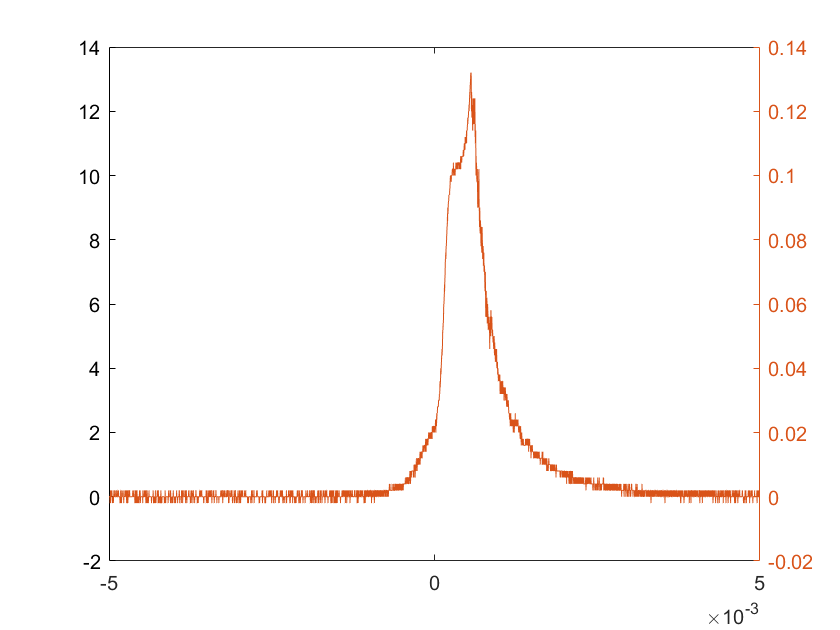
\includegraphics[width = .5\linewidth]{nombredespire.png}
 \caption{$U_1$ (axe de gauche) et $U_2$ (axe de droite) superposés}
 \label{nombredespire}
 \end{figure}
 
 \begin{equation}
     \frac{U_1}{U_2} = \frac{N_1}{N_2} \Leftrightarrow N_1 = \frac{U_1\cdot N_2}{U_2} = \frac{13V \times 5}{0,13V} = 500
 \end{equation}
 
 \subsubsection*{Mesure de l'entrefer maximum}
 
 Cette mesure est faire pour avoir une référence lors du calcul de l'entrefer $e$ avec la mesure de tension. On mesure d'abord le débattement $D$ dans la partie fixe puis l'épaisseur $E$ de la partie mobile.
 
 \begin{equation}
     e_{max} = \frac{D-E}{2} = 1,5\times 10^{-4} m
 \end{equation}
 
 \subsubsection{Étude théorique}
 
 Lorsqu'on actionne l'interrupteur on observe un bref pic de tension aux bornes de la bobine (mesure faite à l'osciloscope, figure \ref{tensionobine}).
 
 \begin{figure}[h!]
 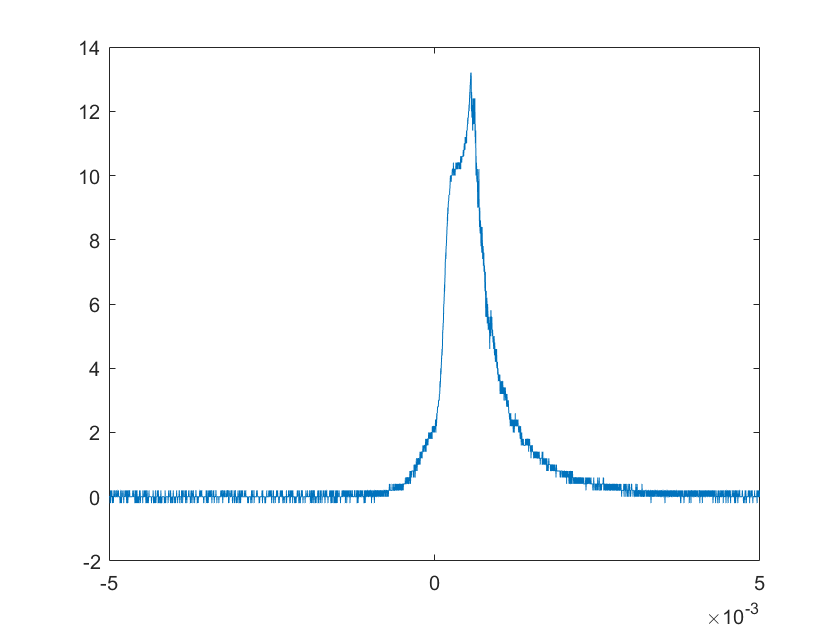
\includegraphics[width = .5\linewidth]{tension.png}
 \centering
 \caption{Tension ($Volts$) en fonction du temps ($secondes$)}
 \label{tensionobine}
 \end{figure}
 
 Avec ces données on peut directement obtenir le flux total \textit{"vu"} par la bobine avec la Loi de Lenz (Figure \ref{fluxobine}):
 
 \begin{equation}
 \Phi_{tot}(t) = -\int U(t) dt
 \end{equation}
 
 \begin{figure}[h!]
 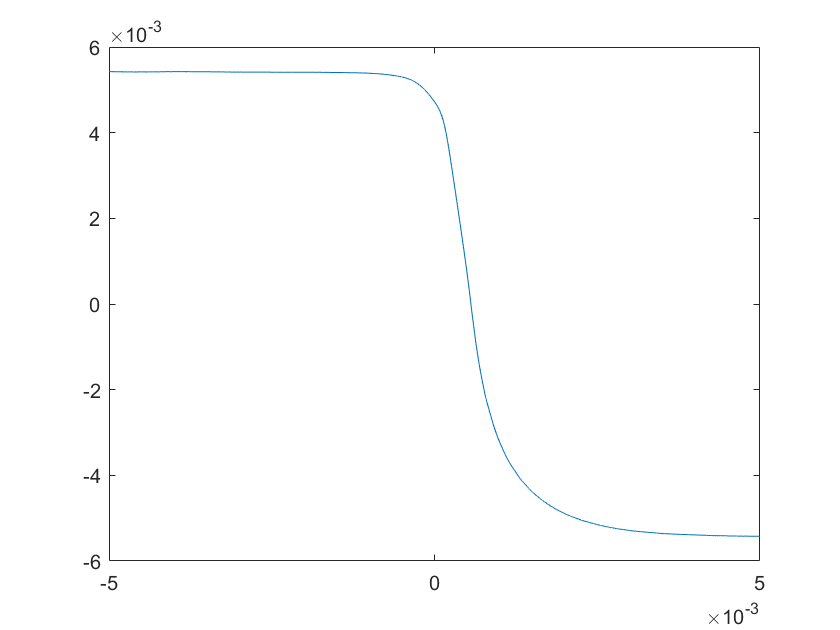
\includegraphics[width = .5\linewidth]{flux.png}
 \centering
 \caption{Flux ($Wb$) en fonction du temps ($secondes$)}
 \label{fluxobine}
 \end{figure}
 
 Puis avec la définition du flux magnétique on obtient le champ magnétique (Figure \ref{champ}): 
 
 \begin{equation}
 \Vert \overrightarrow{B}(t) \Vert = \frac{\Phi_{tot}(t)}{N \cdot dS}
 \end{equation}
 
 \begin{figure}[h!]
 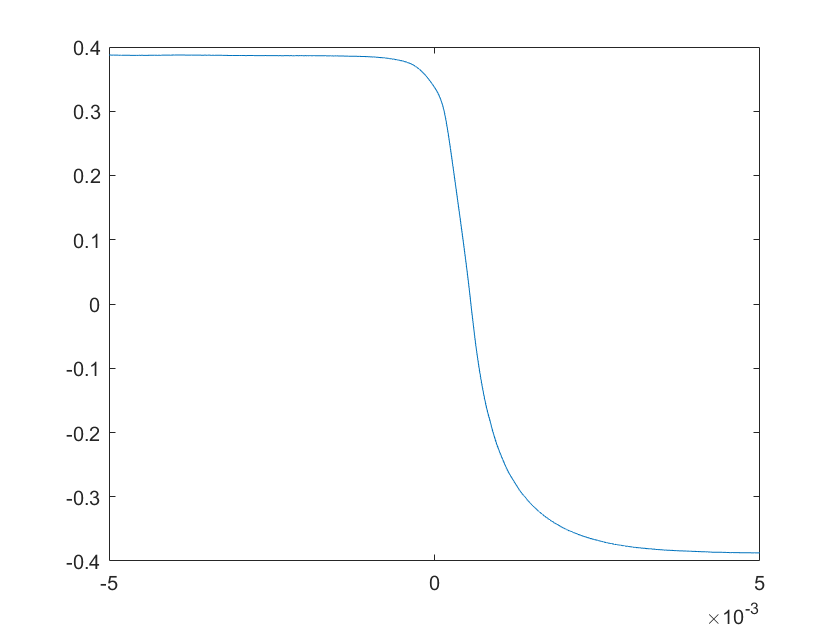
\includegraphics[width = .5\linewidth]{champmag.png}
 \centering
 \caption{Champ magnétique ($T$) en fonction du temps ($secondes$)}
 \label{champ}
 \end{figure}
 
 Avec $N$ le nombre de spire dans la bobine obtenue avec le protocole suivant :
 
On enroule un nombre connu de spires sur le circuit magnétique puis on actionne l'interrupteur en relevant les pics de tension aux bornes des deux enroulements. On déduis le nombre de spires avec le rapport des valeurs des pics et le nombre de spires du second enroulement.

On peut en suite déduire l'entrefer en supposant que la perméabilité du fer est très grande devant celle du vide et donc négligeable :

 \begin{equation}
 e(t) = \frac{\mu_0 \cdot dS}{\Phi_{tot}(t)}
 \end{equation}
 
 \subsection{Convertisseur optique-électronique}
 \paragraph{Énergie disponible}
 Si l'on considère en première approximation que l'éclairage d'une pièce fournie environ $6W/m^2$, un panneau solaire de surface $5cm$ x $1cm$  avec un rendement de $20\%$. On trouve alors une puissance instantanée disponible de l'ordre du milliWatt.Ce qui sur une journée représente une énergie disponible importante au vue des puissance nécessaire de annoncé par le constructeur inférieur au milliWatt.
 
 \subsubsection{Théorie sur les panneaux solaires}
D'après la théorie sur un modèle (Figure \ref{fig:schema_pv}),le panneau solaire peut être représenter par un générateur de courant dont le courant fournie ($Icc$) est proportionnelle à la surface éclairé et à l'irradiance.De plus il y  a une diode en parallèle qui représente le courant dans le noir dû à des effets thermique ($Vd$) en partie puis une résistance en parallèle ($R_{SH}$) et une en série ($R_{S}$) fixant la tension à vide et la tension en courts circuit du panneau solaire.\\

\begin{figure}[h!]
    \centering
    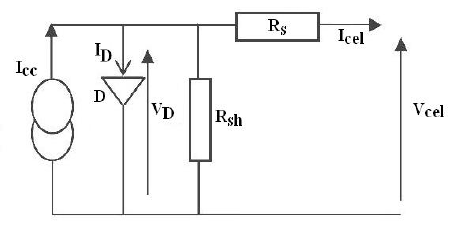
\includegraphics[width=0.9\linewidth]{schema_pv.png}
    \caption{Schéma électrique équivalent d'un panneau solaire}
    \label{fig:schema_pv}
\end{figure}

Ce modèle permet de tracer la caractéristique d'un panneau solaire ($I_{cel}$ en fonction de $V_{cel} $). Cette caractéristique montre une tension constante puis tombe rapidement à zéro à l'approche du courant de cour-circuit et la tension est nul lorsque que le courant de court-circuit est atteint(Figure \ref{fig:caracteristique_pv}). De plus ce courant de court circuit évolue avec l'irrandiance  à l'opposé de la tension en circuit ouvert qui est dépendent très peu de l'irrandiance.

\begin{figure}[h!]
    \centering
   
    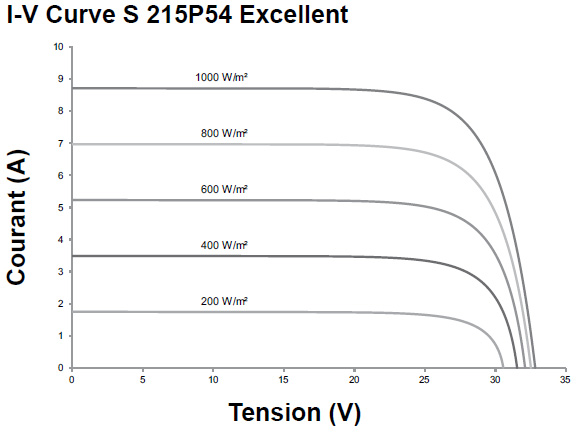
\includegraphics[width=0.7\linewidth]{caracteristique_pv.jpg}
    \caption{Caractéristique théorique d'un panneau solaire}
    \label{fig:caracteristique_pv}
    
\end{figure}

La théorie et le calcul grossier de puissance disponible permettent de justifier l'utilisation d'une panneau solaire pour servir d'alimentation au dispositif \textit{EnOcean} au vue des puissance annoncées par le constructeur.

 \subsubsection{Choix du constructeurs}
 Les panneaux solaires sont utilisés par le constructeur sur les capteurs(Figure \ref{fig:capteur_pv}) afin de remplir la fonction de contraintes sur la récupération d'énergie. Les caractéristiques du panneau solaire monté sur ces capteurs sont disponibles dans la documentation techniques du fabricant, la puissance maximal d'un panneau solaire étant inférieur à $V_{operating} \cdot I_{operating} =3\cdot 4.5\cdot 10^{-6} = 14\mu W$ . La valeur maximal de puissance est donc inférieur aux valeurs annoncées par le constructeur.
 
 \begin{figure}[h!]
     \centering
      \begin{minipage}[c]{0.5\linewidth}
     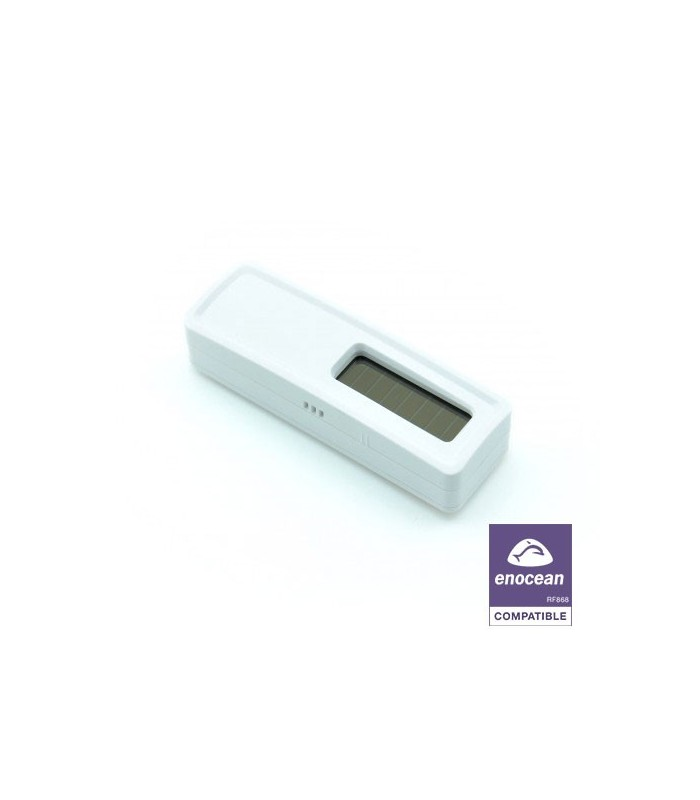
\includegraphics[width=0.7\linewidth,height=5cm] {capteur_pv.jpg}
     \caption{Capteur de température \textit{Enocean} utilisant un panneau solaire}
     \label{fig:capteur_pv}
     \end{minipage}\hfill
      \begin{minipage}[c]{0.5\linewidth}
     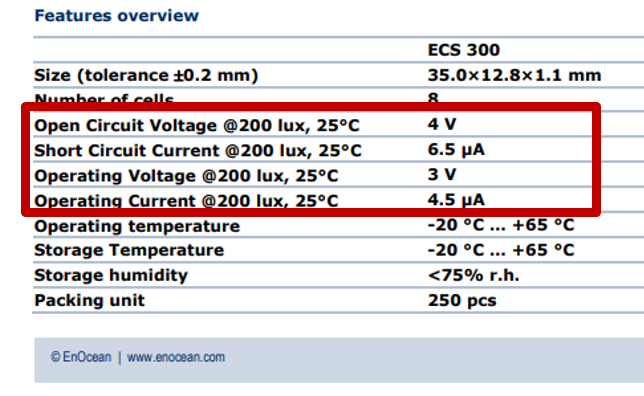
\includegraphics[width=0.9\linewidth,height=5cm]{doc_pv.png}
     \caption{Documentation technique  \textit{Enocean}}
     \label{fig:doc_pv}
     \end{minipage}\hfill
 \end{figure}
 
 \subsubsection{Expérience}
 Une expérience à était réaliser afin de vérifier les caractéristique du panneau solaire proposé par le fabricant.Le problème pour une expérience sur ce panneau est que les valeurs de courants à mesurer sont beaucoup trop faibles par rapport à la précision des instruments disponibles. L'étude à donc était faites sur un panneau solaire plus grand et une loi d'échelle permettra de raccrocher l'expérience au panneau du constructeur.
  \subsubsection*{Protocole}
 Le protocole choisit est de brancher le panneau solaire en parallèle d'un condensateur afin de lisser les valeurs puis sur un bras de pont piloter avec un rapport cyclique $\alpha$ .Entre le point milieu du bras de pont est la masse du circuit, il y a de connecter une charge formée par une résistance et une bobine. Avec ce montage (Figure \ref{fig:exp}) si on fait varier le rapport cyclique du bras de pont, la résistance vue par le panneau solaire varie.Ceci permis donc de parcourir une grande partie de la caractéristique du panneau solaire. Les caractéristique du panneau solaire dépendant aussi de l'irradiance celle-ci sera mesurée par un luxmètre. L'expérience à était réaliser sous trois éclairement, 1 du soleil et 2 en intérieur sous des lumières artificielles.
 
 \begin{figure}[h!]
     \centering
     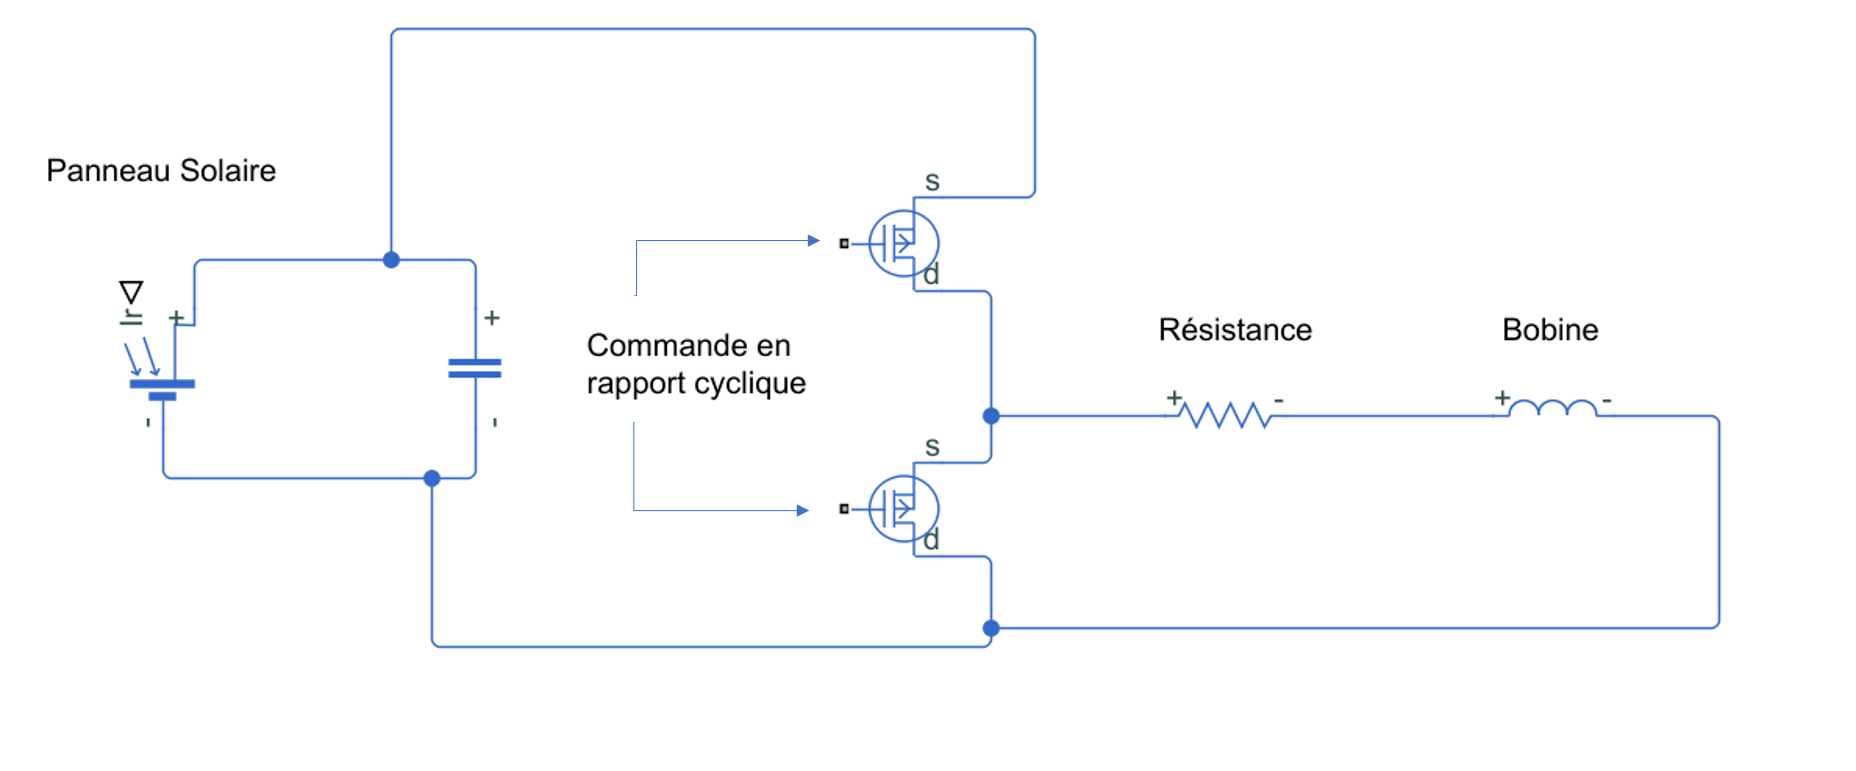
\includegraphics[width=0.9\linewidth]{exp_montage.png}
     \caption{Montage de l'expérience}
     \label{fig:exp}
 \end{figure}
 
 \subsubsection*{Résultats}
 
 A partir des mesures réalisées lors de l'expérience, la caractéristique du panneau solaire(figure \ref{fig:plot_exp} ) mise en évidence est analogue à la théorie à ceci prés que le courant de court circuit n'est pas linéaire avec l'irradiance.
 
 \begin{figure}[h!]
     \centering
     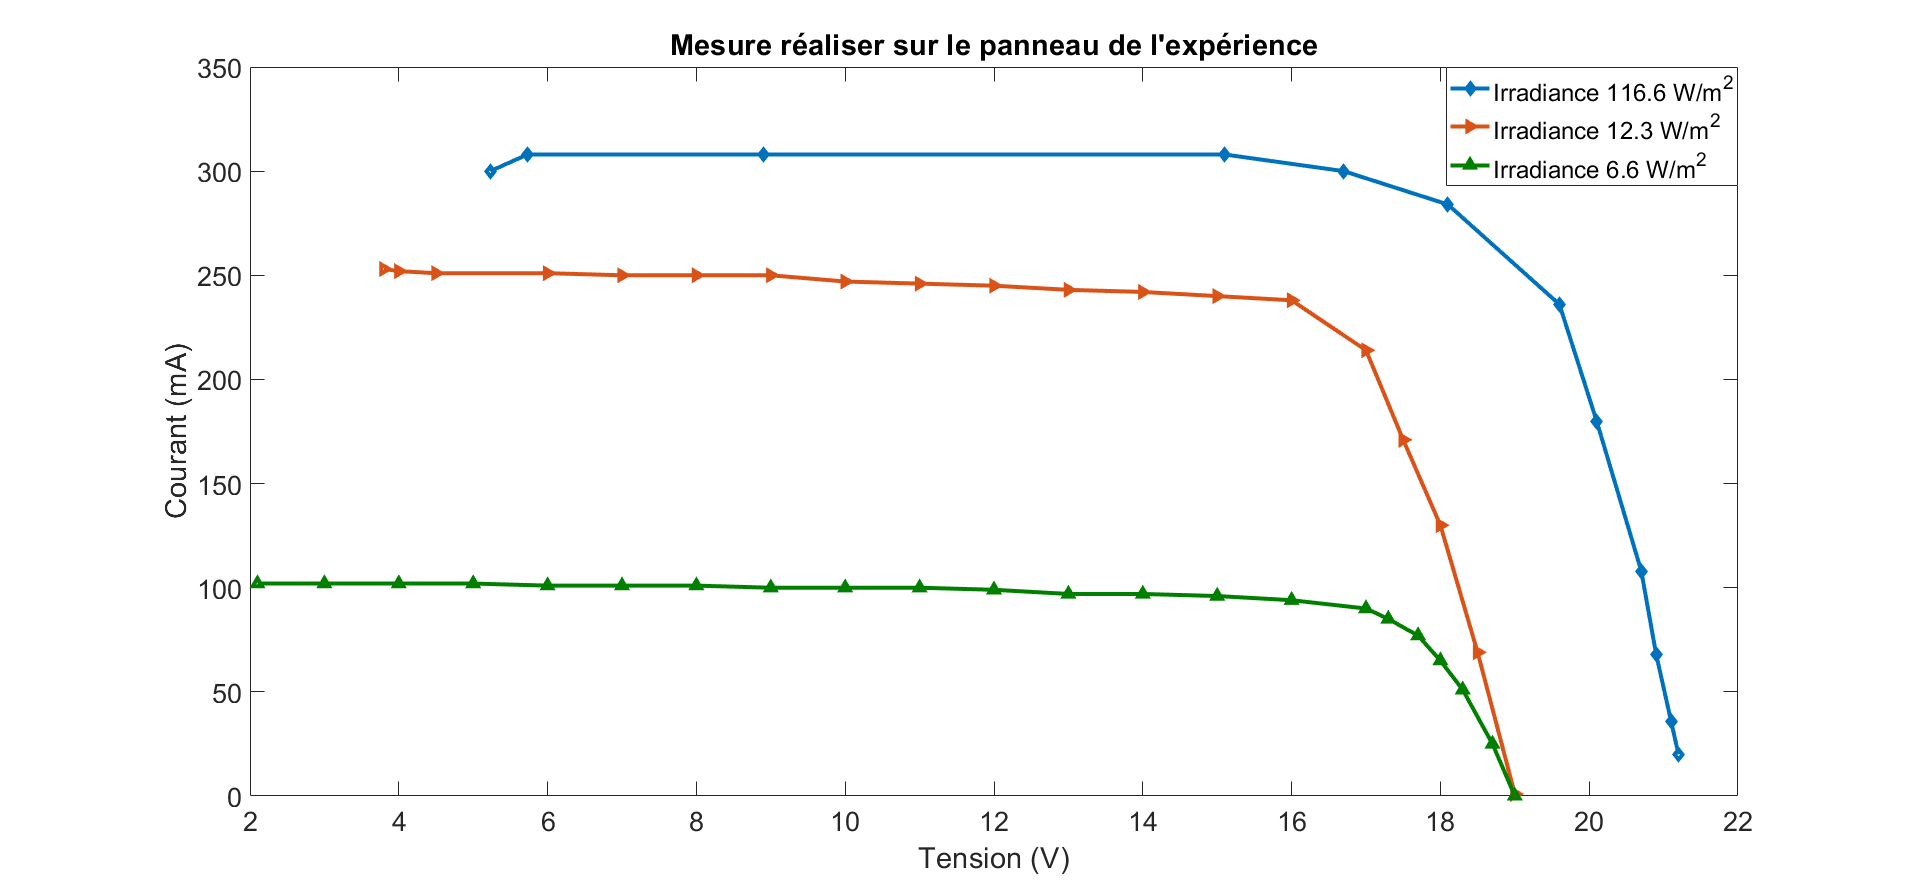
\includegraphics[width=\linewidth]{plot_exp.png}
     \caption{Caractéristique du panneau solaire utilisé pour l'expérience}
     \label{fig:plot_exp}
 \end{figure}
 
 
 \paragraph{Exploitation} Une loi d'échelle permet de raccrocher les valeurs mesurés aux valeurs fournit par le panneau solaire présent sur les modules \textit{EnOcean}.Ceci en ramenant la tension en circuit ouvert celle donné dans la documentation, puis en appliquant le rapport des surfaces éclaires sur  le courant, afin de se rapprocher de la caractéristique supposé du panneau solaire fournit par le fabriquant(figure \ref{fig:plot_enocean}).
 
 \begin{figure}[h!]
     \centering
     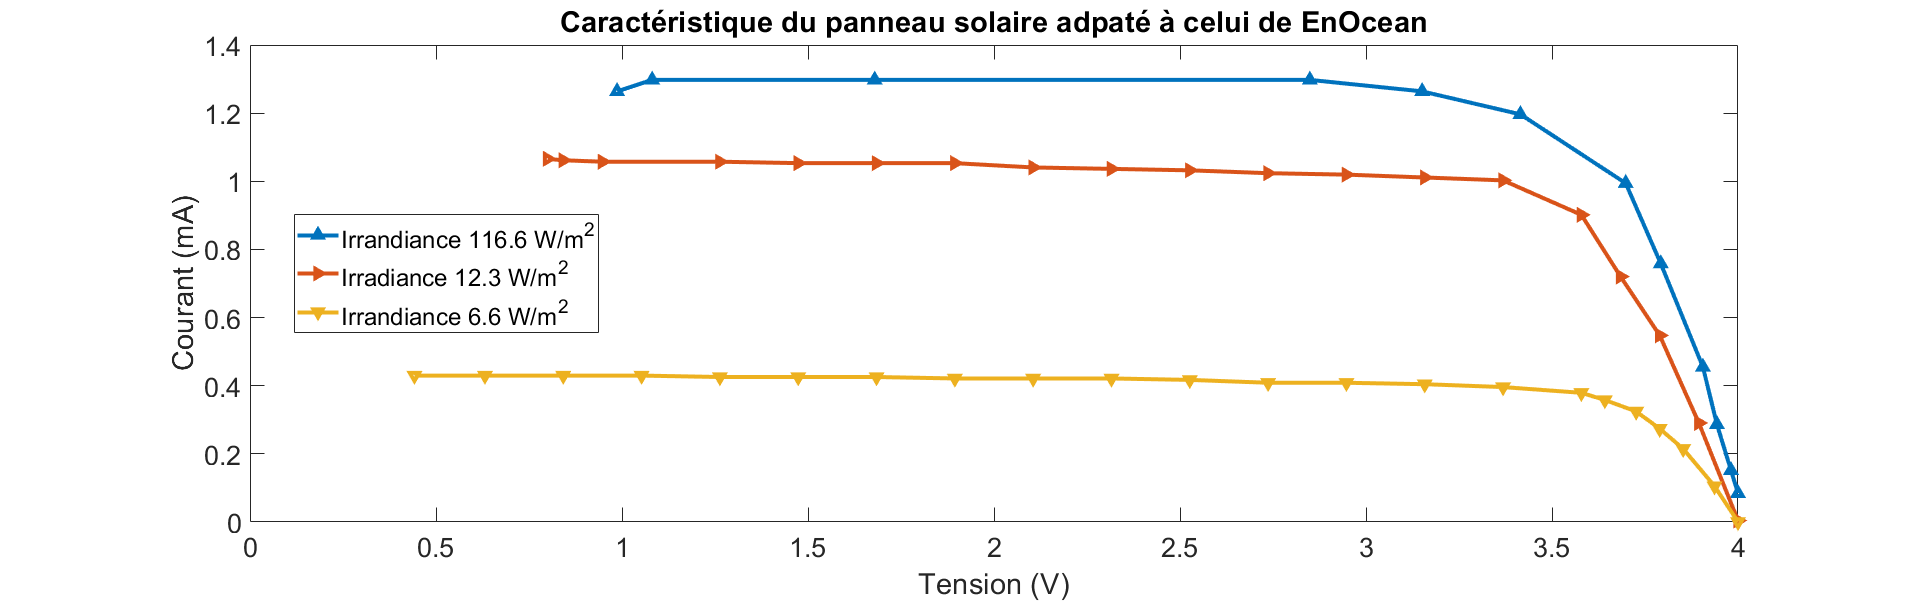
\includegraphics[width=\linewidth]{plot_enocean.png}
     \caption{Caractéristique du panneau solaire mise a l'échelle}
     \label{fig:plot_enocean}
 \end{figure}
 
 
 
 
 \paragraph{Analyses}La non linéarité  peut s'expliquer par la répartition spectrale de la source lumineuse(figure  \ref{fig:spectre_soleil}-\ref{fig:halogène} ) car le silicium répond de manière différente en fonction de la longueur d'onde de la lumière incidente(figure \ref{fig:silicium}).
 
  \begin{figure}[h!]
     \centering
      \begin{minipage}[c]{0.5\linewidth}
      \centering
     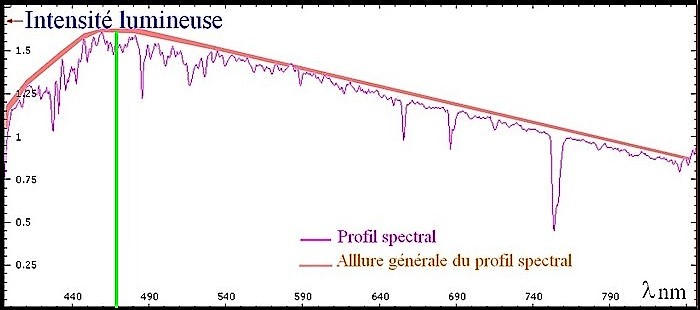
\includegraphics[width=0.9\linewidth]{spectre_soleil.jpg}
     \caption{Spectre du soleil}
     \label{fig:spectre_soleil}
     \end{minipage}\hfill
      \begin{minipage}[c]{0.5\linewidth}
      \centering
     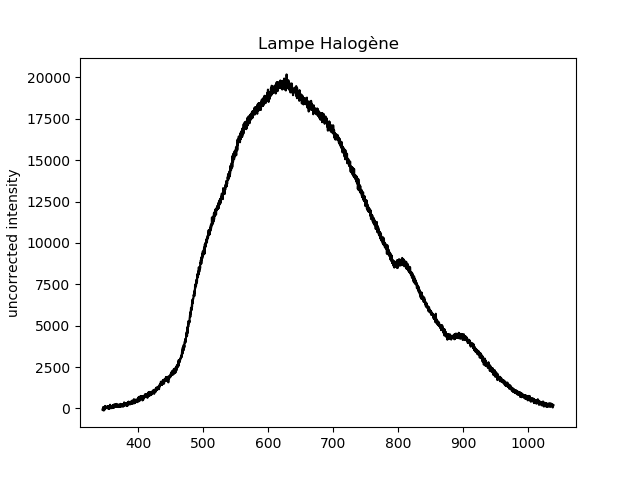
\includegraphics[width=0.9\linewidth,height=5cm]{halogene.png}
     \caption{Spectre lampe d'intérieur halogène utilisé pour l'expérience}
     \label{fig:halogène}
     \end{minipage}\hfill
 \end{figure}
 
 \begin{figure}[h!]
     \centering
     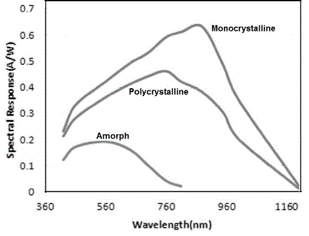
\includegraphics [scale=1]{silicium.png}
     \caption{Réponse spectrale du silicium en fonction de la technologie et de la longueur d'onde}
     \label{fig:silicium}
 \end{figure}

 Il y a aussi après la loi d'échelle une différence avec les valeurs attendus pour le courant de court-circuit. En convertissant sans précision sur la longueur d'onde les $200lux$ en $W/m^2$ puis avec un relation de proportionnalité entre le courant et l'irradiance, la valeur du courant de court-circuit serait donc $20\mu A$ sous $200lux$ pour une valeur attendu de $6.5\mu A$  soit un écart relatif de $208\%$. Cette écart peut être du a la différence technologique entre le panneaux étudié (polycristalin) et  le panneau du kit (monocristalin) ainsi qu'aux sources utilsé pour les mesures car il y a un manque d'informations sur les $200lux$ annoncé notamment sur la longueur d'onde utilisé lors de la mesure par le fabriquant. 
 
 \subsubsection{Conclusion}
 La conclusion de cette étude sur le panneau est qu'il y a des problèmes lors de la loi d'échelle et un manque d'informations sur la mesure effectué par le fabriquant. Malgré cela, si le panneau solaire suit une caractéristique proche de celle mis à l'échelle alors le panneau solaire suffit à fournir la puissance voulue pour le fonctionnement des dispositifs utilisant cette technologie pour la récupération d'énergie.
 
 \section{Réseaux}
 \subsection{Réseaux}
 \subsubsection{Type de réseaux}
 \begin{figure}
     \centering
     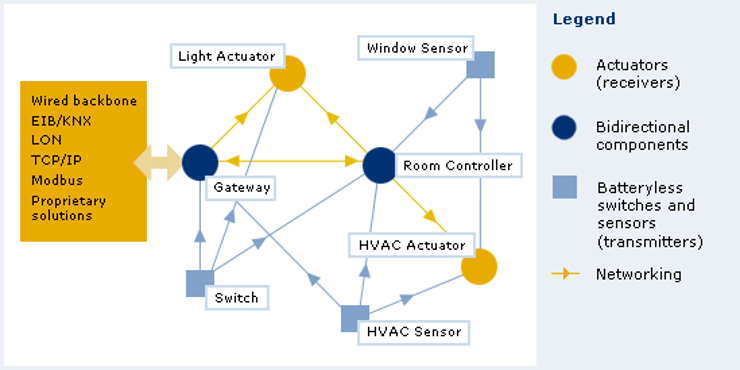
\includegraphics{resseaux.gif}
     \caption{Caption}
     \label{fig:my_label}
 \end{figure}
 
 \subsubsection{Protocoles}
 Le protocole de transmission sans fils utilisé par \textit{EnOcean} est un protocole développé par eux pour les besoins de ces kits de domotique avec récupération d'énergie. Ce protocole est à l'origine d'une norme pour les ensembles domotique similaires: ISO/IEC 14543-3-10. Ce protocoles définit que les communications sont très courtes et souvent unidirectionnelle ainsi que les fréquences utilisés en fonction de la région du monde ($868 Mhz$ pour l'Europe et la Chine et $315Mhz$ pour les États-Unies et le Japon) afin de limiter les interférences et assurant une bonne portée pour l'utilisation.  
 

 \subsection{Caractéristique de la transmission sans fils}
 
 
 \part{Conclusion}
 
 \part{Bibliographie}
\end{document}